\chapter{La récursivité}
{ }\hfill\textbf{Niveau:} moyen\\ \\
\noindent Le langage Logo utilise très souvent une technique de programmation appelée la récursivité. Dans ce chapitre, nous découvrirons tout d'abord cette notion sur des exemples simples pour ensuite approfondir avec notamment le tracé d'une fractale appelée  le flocon de Van Koch. Pour commencer, petite explication:
\begin{center}
\textbf{Une procédure est récursive si elle s'appelle elle-même.}                                                                 \end{center}
\section{Avec la zone de dessin.}
\subsection{ Premier exemple:}
\begin{verbatim}
pour ex1
td 1
ex1
fin  
\end{verbatim}
Cette procédure est récursive puisque la procédure \texttt{ex1} est appelée à la dernière ligne. A l'exécution, on constate que la tortue ne cesse de tourner sur elle-même. Pour interrompre le programme, on est obligé de se servir du bouton STOP.
\subsection{Deuxième exemple:}
\noindent Tout d'abord, voici trois nouvelles primitives:
\begin{itemize}
\item [$\bullet$] \texttt{attends nombre}\hspace {4cm } \textcolor{red}{ \texttt{attends 60}}\\
Bloque le programme pendant le nombre de 60$^{\textrm{ième}}$ de secondes indiqué. \\
Par exemple, \texttt{attends 120} bloquera le programme pendant deux secondes.
\item [$\bullet$] \texttt{gomme}\hspace {4cm } \textcolor{red}{{gomme}}\\
Lorsque la tortue se déplace, elle efface tout au lieu de laisser un trait derrière elle.
\item [$\bullet$] \texttt{dessine,de}\hspace {4cm } \textcolor{red}{{dessine}}\\
Repasse en mode dessin classique: la tortue laisse un trait derrière elle en se déplaçant.
\end{itemize}
\noindent
\begin{verbatim}
pour ex2
av 200 gomme attends 60
re 200 dessine td 6
ex2
fin
\end{verbatim}
Il ne reste plus qu'à lancer ce programme. A chaque seconde le même motif recommence et le programme simule ainsi une trotteuse!
\section{Avec la zone de texte}
\subsection{Un premier exemple:}
\noindent La primitive \texttt{ecris, ec} permet d'afficher un texte dans la zone de texte. elle attend pour argument soit une liste soit un mot. Ex: \texttt{ec "bonjour} \texttt{ec [J'écris ce que je veux]} (Ne pas oublier la quote " lorsqu'on veut juste écrire un mot.)
\begin{verbatim}
pour ex3 :n
ecris :n
ex3 :n+1
fin
\end{verbatim}
Lancer la commande \texttt{ex3 0} puis interrompre avec le bouton STOP\\
Faites les changements nécessaires dans ce programme pour que les chiffres apparaissent de deux en deux.\\
\\
Je veux à présent afficher tous les chiffres supérieur à 100 qui sont dans la table de cinq. Il suffit alors de modifier le programme ainsi:
\begin{verbatim}
pour ex3 :n
ecris :n
ex3 :n+5
fin
\end{verbatim}
 et de lancer: \texttt{ex3 100}
\subsection{Réaliser un test de sortie}
\noindent Taper les commandes suivantes:\\
\texttt{si 2+1=3 [ecris [ceci est vrai]]} \\
\texttt{si 2+1=4 [ecris [ceci est vrai]][ecris [le calcul est faux]]} \\
\texttt{si 2+5=7 [ec "vrai][ec "faux]}\\
\\
Si vous n'avez toujours pas compris la syntaxe de la primtive \texttt{si}, reportez-vous au manuel de référence de \xlogo.
\begin{verbatim}
pour ex3 :n
si :n=100 [stop]
ecris :n
ex3 :n+1
fin
\end{verbatim}
Lancer la commande \texttt{ex3 0}\\
Faites les changements nécessaires dans ce programme pour faire apparaître les chiffres compris entre et 55 et 350 qui sont dans la table de 11.\\
\section{Un exemple de fractale: le flocon de Van Koch}
\noindent Grâce à la récursivité, il est très facile de générer en \logo\ des objets que l'on appelle  en mathématiques des fractales. \\ \\
Voici les premières étapes permettant de créer la ligne brisée de Van Koch. 
\begin{center}
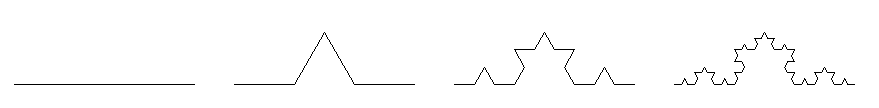
\includegraphics[width=\textwidth]{images/koch0123.png}
\end{center}
Entre chaque étape:
\begin{enumerate}
 \item chacun des segments est partagé en trois parties égales.
 \item on trace un triangle équilatéral sur le deuxième segment.
 \item on efface ce deuxième segment.
\end{enumerate}
\textbf{Ce qu'il faut remarquer:}  Prenons le cas de la deuxième étape, on constate que cette ligne est formée de quatre motifs correspondant à l'étape précédente et dont la taille est divisée par 3. On vient de mettre en évidence la nature récursive de la fractale.\\ \\
Appelons $L_{n,\ell}$ le motif de longueur $\ell$, tracé à l'étape $n$.\\
Pour tracer ce motif voici le procédé:
\begin{enumerate}
 \item On trace $L_{n-1,\ell/3}$
 \item On tourne à gauche de 60 degrés
 \item On trace $L_{n-1,\ell/3}$
 \item On tourne à droite de 120 degrés
 \item On trace $L_{n-1,\ell/3}$
 \item On tourne à gauche de 60 degrés
 \item On trace $L_{n-1,\ell/3}$
\end{enumerate}
En \logo, cela donne tout simplement:
\begin{verbatim}
# :l longueur du motif
# :p étape
pour ligne :l :p
si :p=0 [av :l] [
  ligne :l/3 :p-1 tg 60 ligne :l/3 :p-1 td 120 ligne :l/3 :p-1 tg 60 ligne :l/3 :p-1
]
fin
\end{verbatim}
Si l'on trace un triangle équilatéral composé de trois de ces lignes, on obtient un magnifique flocon de Van Koch
\begin{verbatim}
# :l longueur du côté
pour flocon :l :p
repete 3[ligne :l :p td 120]
fin
\end{verbatim}
Puis en lançant: \texttt{flocon 200 6}
\begin{center}
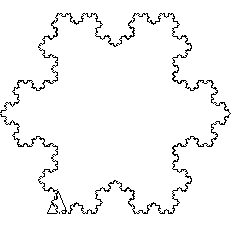
\includegraphics{images/flocon.png}
\end{center}
\section{Recursivite sur les mots}
\noindent Consulter la liste des primitives p.\pageref{liste-prim} afin de comprendre le rôle des primitives \texttt{mot}, \texttt{dernier}, et \texttt{saufdernier}.\\ \\
Voici une procédure récursive qui permet d'inverser l'ordre des lettres d'un mot
\begin{verbatim}
pour inversem :m
si vide? :m [retourne "]  
retourne mot dernier :m inversem saufdernier :m
fin

ecris inversem "abcde
edcba
\end{verbatim}
On dit qu'un mot est un palindrome si on peut le lire dans les deux sens (exemples: radar, laval ...).
\begin{verbatim}
# teste si le mot :m est un palindrome
pour palindrome :m
si  :m=inversem :m [retourne vrai] [retourne faux] 
fin
\end{verbatim}
Et enfin ce joli petit programme (Merci Olivier SC):
\begin{verbatim}
pour palin :n
si palindrome :n [ecris :n stop]
ecris (liste :n "PLUS inversem :n "EGAL somme :n inversem :n)
palin :n + inversem :n 
fin

palin 78
78 PLUS 87 EGAL 165
165 PLUS 561 EGAL 726
726 PLUS 627 EGAL 1353
1353 PLUS 3531 EGAL 4884
4884
\end{verbatim}
\section{Calculer un factorielle}
\label{factorielle}
\noindent On définit factorielle de 5, noté $5!$ par:
 $$5!=5\times4\times3\times2\times1=120$$
De manière générale pour $n$ strictement positif, on remarque que: $n!=n\times(n-1)!$.\\
Cette relation explique la nature récursive de ce programme:
\begin{verbatim}
pour fac :n
si :n=0[ret 1][ret :n*fac :n-1]
fin

ec fac 5
120
ec fac 6
720
\end{verbatim} 
 \section{Une approximation de $\pi$}
\label{approx-pi}
\noindent On peut obtenir une approximation du nombre $\pi$ avec la formule:
$$\pi\approx2^k\sqrt{2-\sqrt{2+\sqrt{2+\ldots\sqrt{2+\sqrt2}}}}$$ où $k$ est le nombre de racines carrées. Plus $k$ devient grand et plus cette expression se rapproche du nombre $\pi$.\\ \\
La formule est constituée de l'expression $2+\sqrt{2+\ldots\sqrt{2+\sqrt2}}$ qui est clairement récursive d'où le programme:
\begin{verbatim}
# k désigne le nombre de racines
pour approxpi :k
tape "Approximation:\  ec (puissance 2 :k) * racine (2- racine (calc :k-2))
ec "-------------------------
tape "Pi:\  ec pi
fin

pour calc :p
si :p=0 [ret 2][ret 2+racine calc :p-1]
fin

approxpi 10
Approximation: 3.141591421568446 
------------------------- 
Pi: 3.141592653589793 
\end{verbatim}
On a obtenu les 5 premières décimales! Si l'on souhaite davantage, il faudra éliminer certaines erreurs de calculs dues aux racines carrées imbriquées. Pour cela nous allons augmenter le nombre de décimales avec la primitive \texttt{fixedecimales}.
\begin{verbatim}
fixedecimales 100
approxpi 100
Approximation: 3.1415926535897932384626433832795028841973393069670160975807684313880468...
------------------------- 
Pi: 3.141592653589793238462643383279502884197169399375105820974944592307816406....
\end{verbatim}
Et on obtient à présent 39 décimales...